\documentclass{article}
\usepackage[margin=1.5in]{geometry}
% ams packages (ESSENTIAL)
\usepackage{amsmath,amsfonts,amssymb,amsthm}
% Allows for inclusion of graphics (pictures)
\usepackage{graphicx}

% Figure displays:
\usepackage{caption}
\usepackage{subcaption}

% Typeface
%\usepackage{mathpazo}

% Code
\usepackage{listings}
\usepackage{color}

 \lstset{frame=tb,
 	language=Java,
 	breaklines=true,
 	showstringspaces=false,
 	columns=flexible,
 	numbers=none,
 	commentstyle=\color{dkgreen},
 	stringstyle=\color{mauve},
 	tabsize=4
 }
 
 \usepackage{tikz}
 

\title{Lab 10: Binary Search Trees}
\author{Sam Harder}

\begin{document}
	\maketitle
	\begin{enumerate}
		\item The smallest height of a BST with 16 nodes is 
		\[ \boxed{\lg (16)  = 4.}  \]
		\item 
		\leavevmode
				\begin{lstlisting}[language=Java]
	public boolean equal(BSTNode t1, BSTNode t2){
	
		if(t1 == null && t2 == null){
			return true;
		}
		else{
			return false;
		}
	
		if( !(t1.getKey().equals(t2.getKey())) ){
			return false;
		}
		
		boolean leftMatch = equal(t1.getLeftNode(), t2.getLeftNode());
		boolean rightMatch = equal(t1.getRightNode(), t1.getRightNode());
		
		return leftMatch && rightMatch;
	}
		\end{lstlisting}
		
		\item See Figure 1.
		\begin{figure}[h]
			\begin{subfigure}{0.6\textwidth}
				\centering
				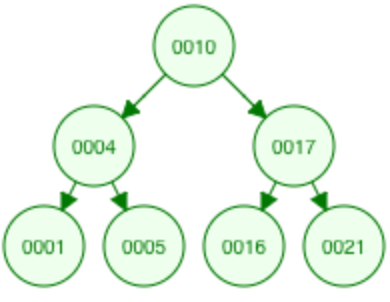
\includegraphics[width=0.6\textwidth]{2level.png}
				\caption{2 Levels}
			\end{subfigure}
			%
			\begin{subfigure}{0.6\textwidth}
				\centering
				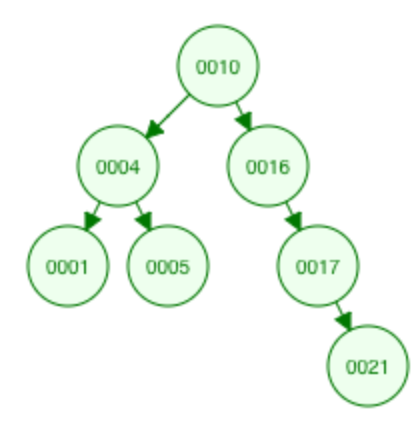
\includegraphics[width=0.6\textwidth]{3level.png}
				\caption{3 Levels}
			\end{subfigure}
			
			\begin{subfigure}{0.6\textwidth}
				\centering
				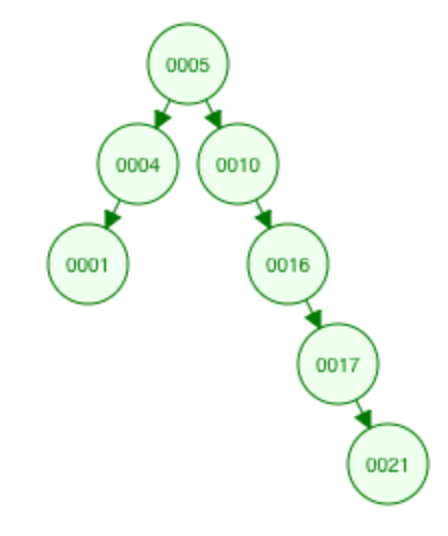
\includegraphics[width=0.6\textwidth]{4level.png}
				\caption{4 Levels}
			\end{subfigure}
			%
			\begin{subfigure}{0.6\textwidth}
				\centering
				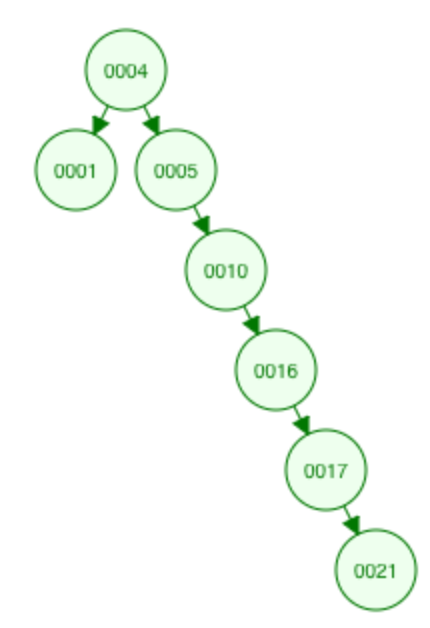
\includegraphics[width=0.6\textwidth]{5level.png}
				\caption{5 Levels}
			\end{subfigure}
			
			\begin{subfigure}{0.6\textwidth}
				\centering
				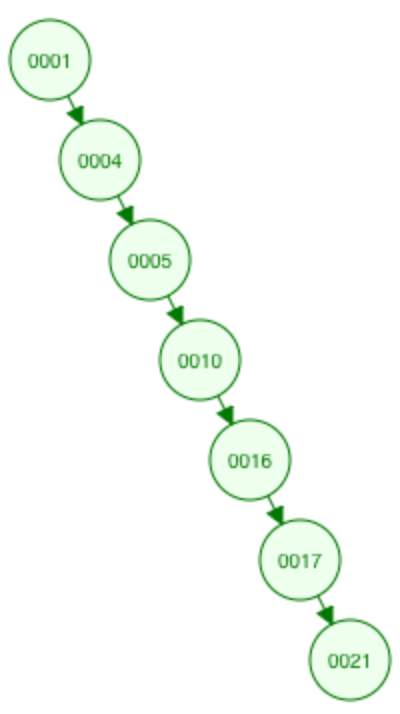
\includegraphics[width=0.5\textwidth]{6level.png}
				\caption{6 Levels}
			\end{subfigure}
			\caption{Different BSTs for \{1,4,5,10,16,17,21\}}
		\end{figure}
		
		\item
		This creates a tree of height $n-1$ where there are no left child nodes, only right child nodes and where there is exactly one leaf. See \textbf{Figure 1(e) } for an example of what this tree would look like. 
		
		\item 
		The central quality of a BST is that at any node $A$, the keys in the right subtree will all be greater than the key of $A$, and the keys in the left subtree will be less than the key of $A$. 
		
		First I would like to show that if a node $A$ has two children then its predecessor will always be in its left subtree. If $A$ does not have a parent, then it follows that $A$ is the root of the tree and all the nodes less than $A$ will be in the left subtree. Since the predessor is less than $A$ it will be in the left subtree. If $A$ does have a parent $B$ then there can exist nodes less than $A$ which are not in $A$'s left subtree. However, if $A$ has a left subtree then there exist nodes that are greater than $B$ but less than $A$. The predecessor is one of those nodes and will therefore be in $A$'s left subtree. 
		
		Next I would like to show that if a node $A$ has two children then its successor will always be in its right subtree. If $A$ does not have a parent, then it follows that $A$ is the root of the tree and all the nodes greater than $A$ will be in the right subtree. Since the successor is greater than $A$ it will be in the right subtree. If $A$ does have a parent $B$ then there can exist nodes greater than $A$ which are not in $A$'s right subtree. However, if $A$ has a right subtree then there exist nodes that are less than $B$ but greater than $A$. The successor is one of those nodes and will therefore be in $A$'s right subtree. 
			
		We wish to prove the statement, \textit{if a node $P$ is a predecessor of $A$ and $A$ has two subtrees, then it has no right node.} We prove it through contradiction. We saw earlier that if $A$ has two subtrees then the node $P$ will always be in the left subtree. If a node $P$ is the predecessor of $A$ and it has a right node, then there must exist a key greater than $P$ which is less than $A$. This contradicts our original statement that $P$ was the predecessor of $A$. Therefore, \textit{if a node $P$ is a predecessor of $A$, then it has no right node.}
		
		We wish to prove the statement, \textit{if a node $P$ is a successor of $A$ and $A$ has two subtrees, then it has no left node.} We prove it through contradiction. We saw earlier that if $A$ has two subtrees then the node $S$ will always be in the right subtree. If $S$ has a left node, then there must exist a key less than $S$ which is greater than $A$. This contradicts our original statement that $S$ was the successor of $A$. Therefore, \textit{if a node $S$ is a successor of $A$ and $A$ has two subtrees, then it has no left node.}
		
		\item 
		The worst case is if the list being inserted is already sorted. In this case each subsequent item inserted is compared to every key already in the tree before being inserted at the end. This means that there are,
		\[  1 + 2 + 3 + \ldots + (n-1) + n = \frac{n(n+1)}{(2)} \]
		comparisions when inserting a sorted list of length $n$ into a binary search tree. Therefore insertion is $O(n^2)$ in the worst case. 
		
		Printing the tree recursively is $O(n)$ regardless of how the tree is built.
		
		Therefore the entire process of insertion and printing is $O(n^2)$ in the worst case. 
					
		\textit{Source: https://en.wikipedia.org/wiki/Tree\_sort}			
		
		\item Unfortunately, Professor Shrub has  \textit{not }discovered a remarkable property of binary search trees. His hypothesis can be disproven with the simple tree of four nodes in \textbf{Figure 2}.
		
		\begin{figure}[h]
			\centering
			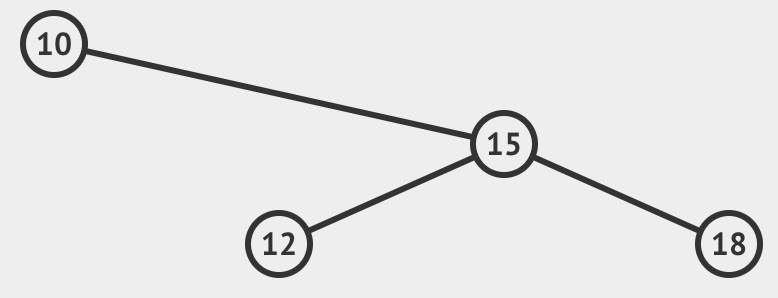
\includegraphics[width=0.5\textwidth]{7.png}
			\caption{Professor Shrub's Downfall}
		\end{figure}.
		
		If we search for the key $18$ in this tree the set $A$ of keys to the left of the search will be
		\[  A = \{12\}, \]
		the set $B$ of keys along the search path will be
		\[  B = \{10, 15, 18  \}  \]
		and the set $C$ of keys to the right of the search path is empty
		\[  C = \{\}.  \]
		
		Note now that $12 \in B$ and $10 \in A$, but $12 \nleq 10$, therefore Professor Shrub's hypothesis is disproven. 
		
		\item No this is not true. Let's consider the tree with four nodes in \textbf{Figure 3. }
		\begin{figure}[h]
			\centering
			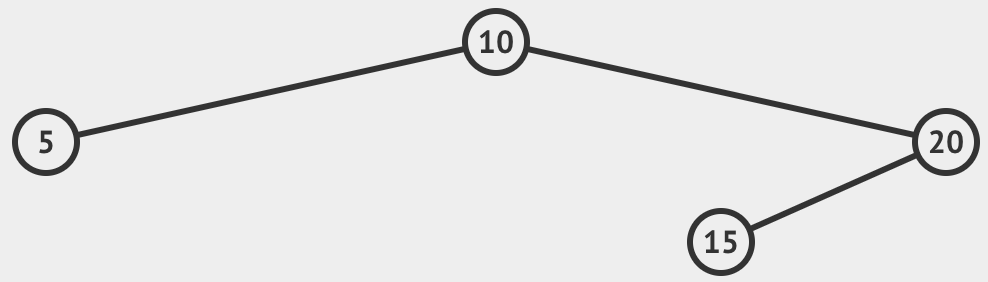
\includegraphics[width=0.5\textwidth]{81.png}
			\caption{Counterexample to Commutativity of Node Removal}
		\end{figure}
		If we remove the node with key 5 and then the node with key 20 we get the tree seen in \textbf{Figure 4},
		\begin{figure}[h]
			\centering
			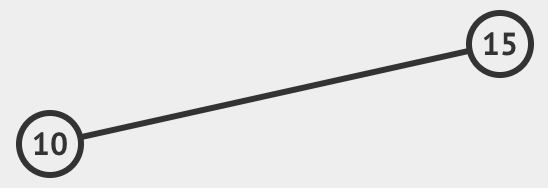
\includegraphics[width=0.5\textwidth]{83.png}
			\caption{Result if one removes 5 then 20}
		\end{figure}
		while if we remove them in the opposite way we get \textbf{Figure 5}.
		\begin{figure}[h]
			\centering
			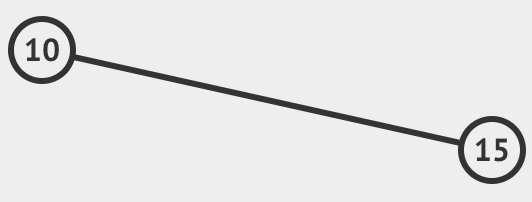
\includegraphics[width=0.5\textwidth]{82.png}
			\caption{Result if one removes 20 then 5}
		\end{figure}
		\end{enumerate}
\end{document}